\documentclass[a4paper]{article}

\usepackage[top=1cm,bottom=1cm,left=1cm,landscape]{geometry}

\usepackage{tikz}
\usetikzlibrary{arrows,arrows.meta}
%\input{arrowsnew}
%% Font setting, for my own eyes
\usepackage{libertine}
\usepackage{libertinust1math}
\usepackage[T1]{fontenc}
\usetikzlibrary{calc}

\begin{document}
	\pagenumbering{gobble}
	\tikzstyle{mbigblock} = [rectangle, draw, text width=13cm, text centered, rounded corners, minimum height=1em]
	\tikzstyle{block}  = [rectangle, draw, text width=3.5cm, text centered, minimum height=1em]
	\tikzstyle{lblock} = [rectangle, draw, text width=5cm, text centered, minimum height=1em]
	\tikzstyle{rblock} = [rectangle, draw, text width=3.5cm, text centered, minimum height=1em]
	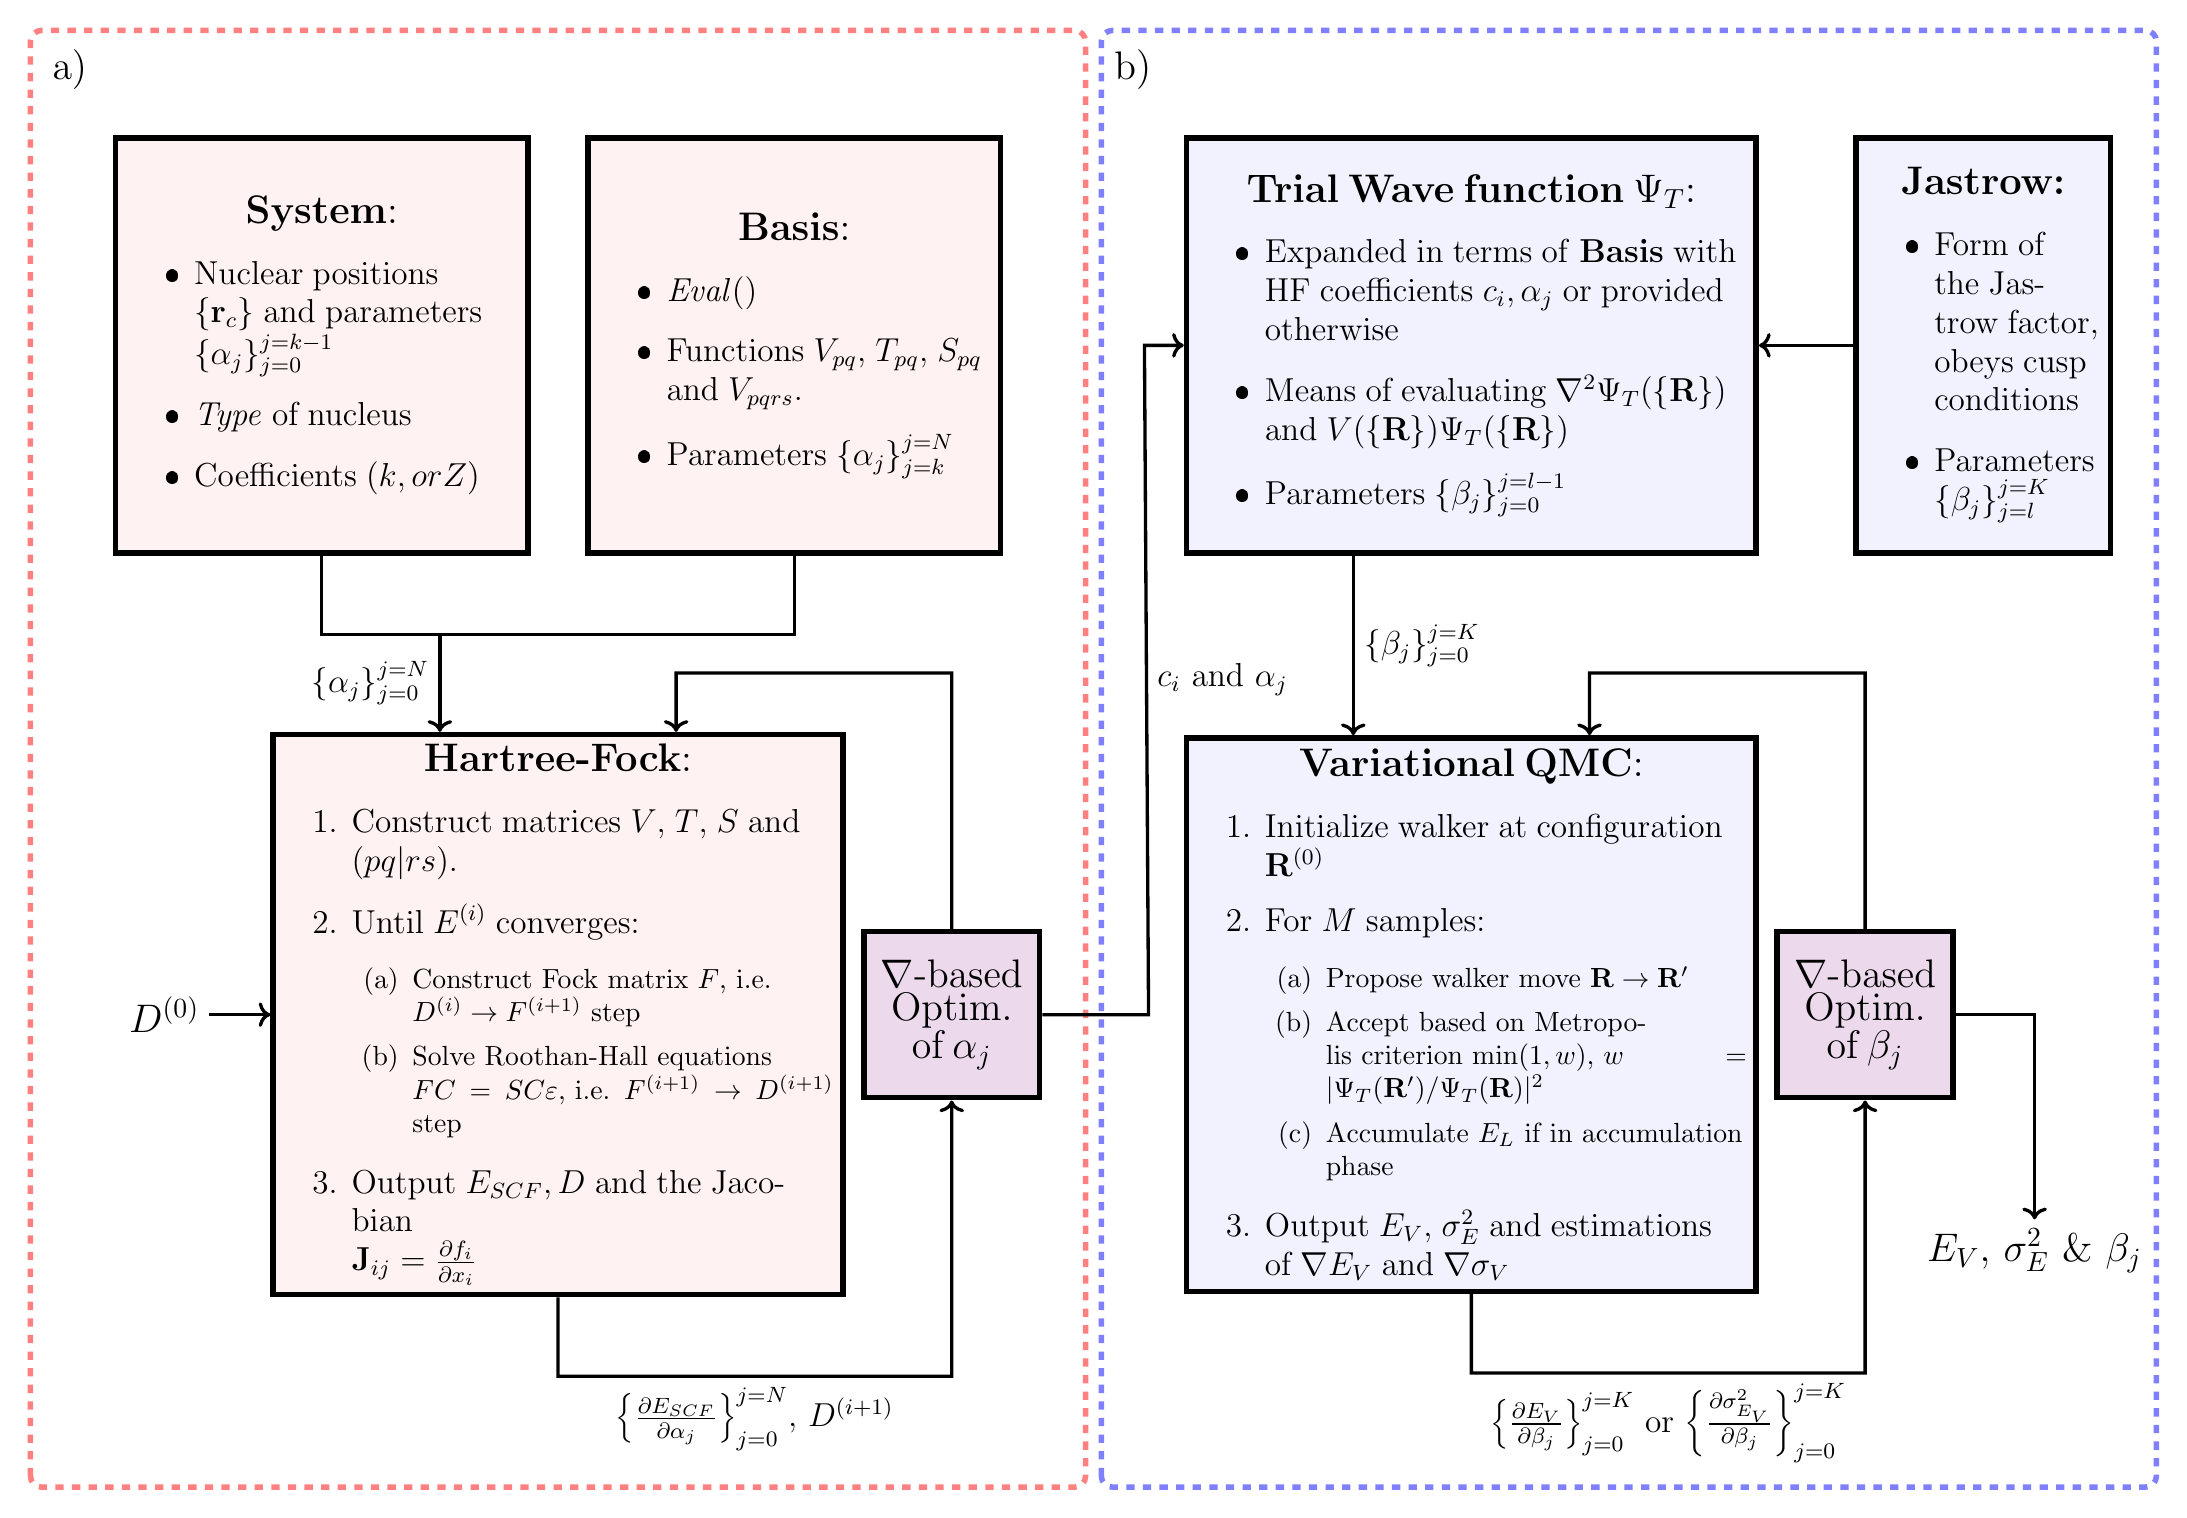
\begin{tikzpicture}[node distance=6.5cm]
%		\draw (0.0,0) rectangle (30cm,21cm);
		% LHS of the diagram, the Hartree-Fock Module
		\draw[color=red!50, line width=2, dashed, rounded corners] (0.0,0) rectangle (13.4cm,18.5cm);
		\draw (0.5, 18.0) node {\Large {a)}};
		
		\node (hf) [rectangle, draw, text width=7cm, align=center, minimum height=20em, line width=2, fill=red!5] at (6.7, 6) 
		{\Large{\textbf{Hartree-Fock}:}
		\large
		\begin{enumerate}
			\item Construct matrices $V$, $T$, $S$ and $(pq|rs)$.
			\item Until $E^{(i)}$ converges:
				   \normalsize
				   {
				   \begin{enumerate}
				   \item Construct Fock matrix $F$, i.e. \\
				   $D^{(i)} \rightarrow F^{(i+1)}$ step
				   \item Solve Roothan-Hall equations \\ $FC = SC\mathbf{\varepsilon}$, i.e. 
				   $F^{(i+1)} \rightarrow D^{(i+1)}$ step
				   \end{enumerate}
  			   	   }
	    	   	   \large
	   	    \item Output $E_{\text{SCF}}, D$ and the Jacobian \\ $\mathbf{J}_{i j}=\frac{\partial f_{i}}{\partial x_{i}}$

		\end{enumerate}
		};
		
		\node (sys) [rectangle, draw, text width=5cm, align=center, minimum height=15em, line width=2, fill=red!5] at (6.7-3, 14.5)
		{\Large{\textbf{System}:}
		\large
		\begin{itemize}
			\item Nuclear positions $\{\mathbf{r}_{c}\}$ and parameters $\{\alpha_j\}_{j=0}^{j=k-1}$
			\item \emph{Type} of nucleus
			\item Coefficients $(k, \text{or } Z)$
		\end{itemize}
		};
	
		\node (basis) [rectangle, draw, text width=5cm, align=center, minimum height=15em, line width=2, fill=red!5] at (6.7+3, 14.5)
		{\Large{\textbf{Basis}:}
		\large
		\begin{itemize}
			\item \emph{Eval}()
			\item Functions $V_{pq}$, $T_{pq}$, $S_{pq}$ and $V_{pqrs}$.
			\item Parameters $\{\alpha_j\}_{j=k}^{j=N}$
		\end{itemize}
		};
	
		\node (inphf) at (6.7-5, 6) {\Large $D^{(0)}$};
	
		\node (opt) [rectangle, draw, text width=2cm, align=center, minimum height=6em, line width=2, fill=violet!15] at (6.7+5, 6) {\Large $\mathbf{\nabla}$-based \\ Optim. of $\alpha_j$};
	
		% Flows
		\draw[very thick, black] (basis.south) --++ (0.0, -1.0cm) --++  ($(sys.south)-(basis.south)$) --++ (0.0, 1.0cm);
		\draw[very thick, black, ->] ($0.5*(basis.south)+0.5*(sys.south)-(1.5cm, 1.0cm)$) -- node[anchor=east] {\large $\{\alpha_j\}_{j=0}^{j=N}$} ($(hf.north)-(1.5cm, 0cm)$);
		\draw[very thick, black, ->] (hf.south) --++ (0.0, -1.0cm) --++  (5.0cm, 0.0cm) node[midway, anchor=north] {\large $\left\{ \frac{\partial E_{\text{SCF}}}{\partial \alpha_j} \right\}_{j=0}^{j=N}$, $D^{(i+1)}$} -- (opt.south);
		\draw[very thick, black, ->] (opt.north) --++ (0.0, 3.25cm) --++  (-3.5cm, 0.0cm) -- ($(hf.north)+(1.5cm, 0cm)$);
		\draw[very thick, black, ->] (inphf) -- (hf.west);
		
		% THS of the diagram, the QMC Module
		\draw[color=blue!50, line width=2, dashed, rounded corners] (13.6,0) rectangle (27cm,18.5cm);		
		\draw (14, 18) node {\Large {b)}};
		\node (vmc) [rectangle, draw, text width=7cm, align=center, minimum height=20em, line width=2, fill=blue!5] at (4.7+13.6, 6) 
		{\Large{\textbf{Variational QMC}:}
			\large
			\begin{enumerate}
				\item Initialize walker at configuration $\mathbf{R}^{(0)}$
				\item For $M$ samples:
				\normalsize
				{
					\begin{enumerate}
						\item Propose walker move $\mathbf{R} \rightarrow \mathbf{R}^\prime$
						\item Accept based on Metropolis criterion $\min (1, w)$, $w=|\Psi_T(\mathbf{R}^{\prime}) / \Psi_T(\mathbf{R})|^{2}$
						\item Accumulate $E_L$ if in accumulation phase
					\end{enumerate}
				}
				\large
				\item Output $E_V$, $\sigma^2_E$ and estimations of $\nabla E_V$ and $\nabla \sigma_V$ 
				
			\end{enumerate}
		};
		\node (vopt) [rectangle, draw, text width=2cm, align=center, minimum height=6em, line width=2, fill=violet!15] at (13.6+4.7+5, 6) {\Large $\mathbf{\nabla}$-based \\ Optim. of $\beta_j$};
		
		\node (psi) [rectangle, draw, text width=7cm, align=center, minimum height=15em, line width=2, fill=blue!5] at (13.6+4.7, 14.5)
		{\Large{\textbf{Trial Wave function $\Psi_T$}:}
			\large
			\begin{itemize}
				\item Expanded in terms of \textbf{Basis} with HF coefficients $c_i, \alpha_j$ or provided otherwise
				\item Means of evaluating $\nabla^2 \Psi_T(\{\mathbf{R}\})$ and $V(\{\mathbf{R}\}) \Psi_T(\{\mathbf{R}\})$
				\item Parameters $\{\beta_j\}_{j=0}^{j=l-1}$
			\end{itemize}
		};
		
		\node (jast) [rectangle, draw, text width=3cm, align=center, minimum height=15em, line width=2, fill=blue!5] at (13.6+11.2, 14.5)
		{\Large{\textbf{Jastrow:}}
			\large
			\begin{itemize}
				\item Form of the Jastrow factor, obeys cusp conditions
				\item Parameters $\{\beta_j\}_{j=l}^{j=K}$
			\end{itemize}
		};
	
		\node (out) at ($(vopt.east)+(1.0, -3.0)$) {\Large $E_{\text{V}}$, $\sigma^2_E$ \& $\beta_j$};
	
		% Flows
		\draw[very thick, black, ->] (opt) --++ (2.5, 0.0) -- ($(psi.west)-(0.5, 0.0)$) node[midway, anchor=west] {\large $c_i$ and $\alpha_j$} -- (psi.west);
		\draw[very thick, black, ->] (vmc.south) --++ (0.0, -1.0cm) --++  (5.0cm, 0.0cm) node[midway, anchor=north] {\large $\left\{ \frac{\partial E_{\text{V}}}{\partial \beta_j} \right\}_{j=0}^{j=K}$ or $\left\{ \frac{\partial \sigma^2_{E_{V}}}{\partial \beta_j} \right\}_{j=0}^{j=K}$} -- (vopt.south);
		\draw[very thick, black, ->] (jast.west) -- (psi.east);
		\draw[very thick, black, ->] (vopt.north) --++ (0.0, 3.25cm) --++  (-3.5cm, 0.0cm) -- ($(vmc.north)+(1.5cm, 0cm)$);
		\draw[very thick, black, ->] ($(psi.south)-(1.5cm, 0cm)$) -- node[midway, anchor=west] {\large $\{\beta_j\}_{j=0}^{j=K}$} ($(vmc.north)-(1.5cm, 0cm)$);
		\draw[very thick, black, ->] (vopt.east) --++ (1.0 ,0.0) -- (out.north);
		
	\end{tikzpicture}
\end{document}

